% coding:utf-8
\section{Kettenlinie}
Aufgabenstellung: 
\[y(x) = a \cdot \cosh\left(\frac{x}{c}\right) + b\]
a)\\
\[h = H - y(x) = y(\ell) - y(x)\]
\[h = a \cosh\left(\frac{\ell}{c}\right) + b - \left(a \cosh\left(\frac{x}{c}\right) + b\right)\]
\[h = a \cdot \cosh\left(\frac{\ell}{c}\right) - a \cdot \underbrace{\cosh\left(\frac{x}{c}\right)}_1\]
\[\rightarrow x = 0\]
\[\Rightarrow h_{max} = a \cdot \cosh\left(\frac{\ell}{c}\right)-a\]
\[\underline{\underline{h(\ell) = a \cosh\left(\frac{\ell}{c}\right) - 10}}\]
b)
\[h(\ell_1) =a \cdot \cosh\left(\frac{\ell}{c}\right) - 10\]
\[\cosh\left(\frac{\ell}{c}\right) = \frac{h(\ell_1 + a}{a}\]
\[\Rightarrow \underline{\underline{\arccosh\left(\frac{h(\ell_1 + a}{a}\right) \cdot a}}\]
c)
\[m(\ell) = h'(\ell) = \sinh\left(\frac{\ell}{c}\right)\]
\[m(\ell) = \tan(\beta) \quad\]
\[\Rightarrow \underline{\underline{\alpha = \frac{\pi}{2} - \beta = \frac{\pi}{2} - \arctan(m(\ell)) = \frac{\pi}{2} - \arctan(\sinh\left(\frac{\ell}{c}\right))}}\]
\section{Maximale Fläche}
Aufgabenstellung: \\
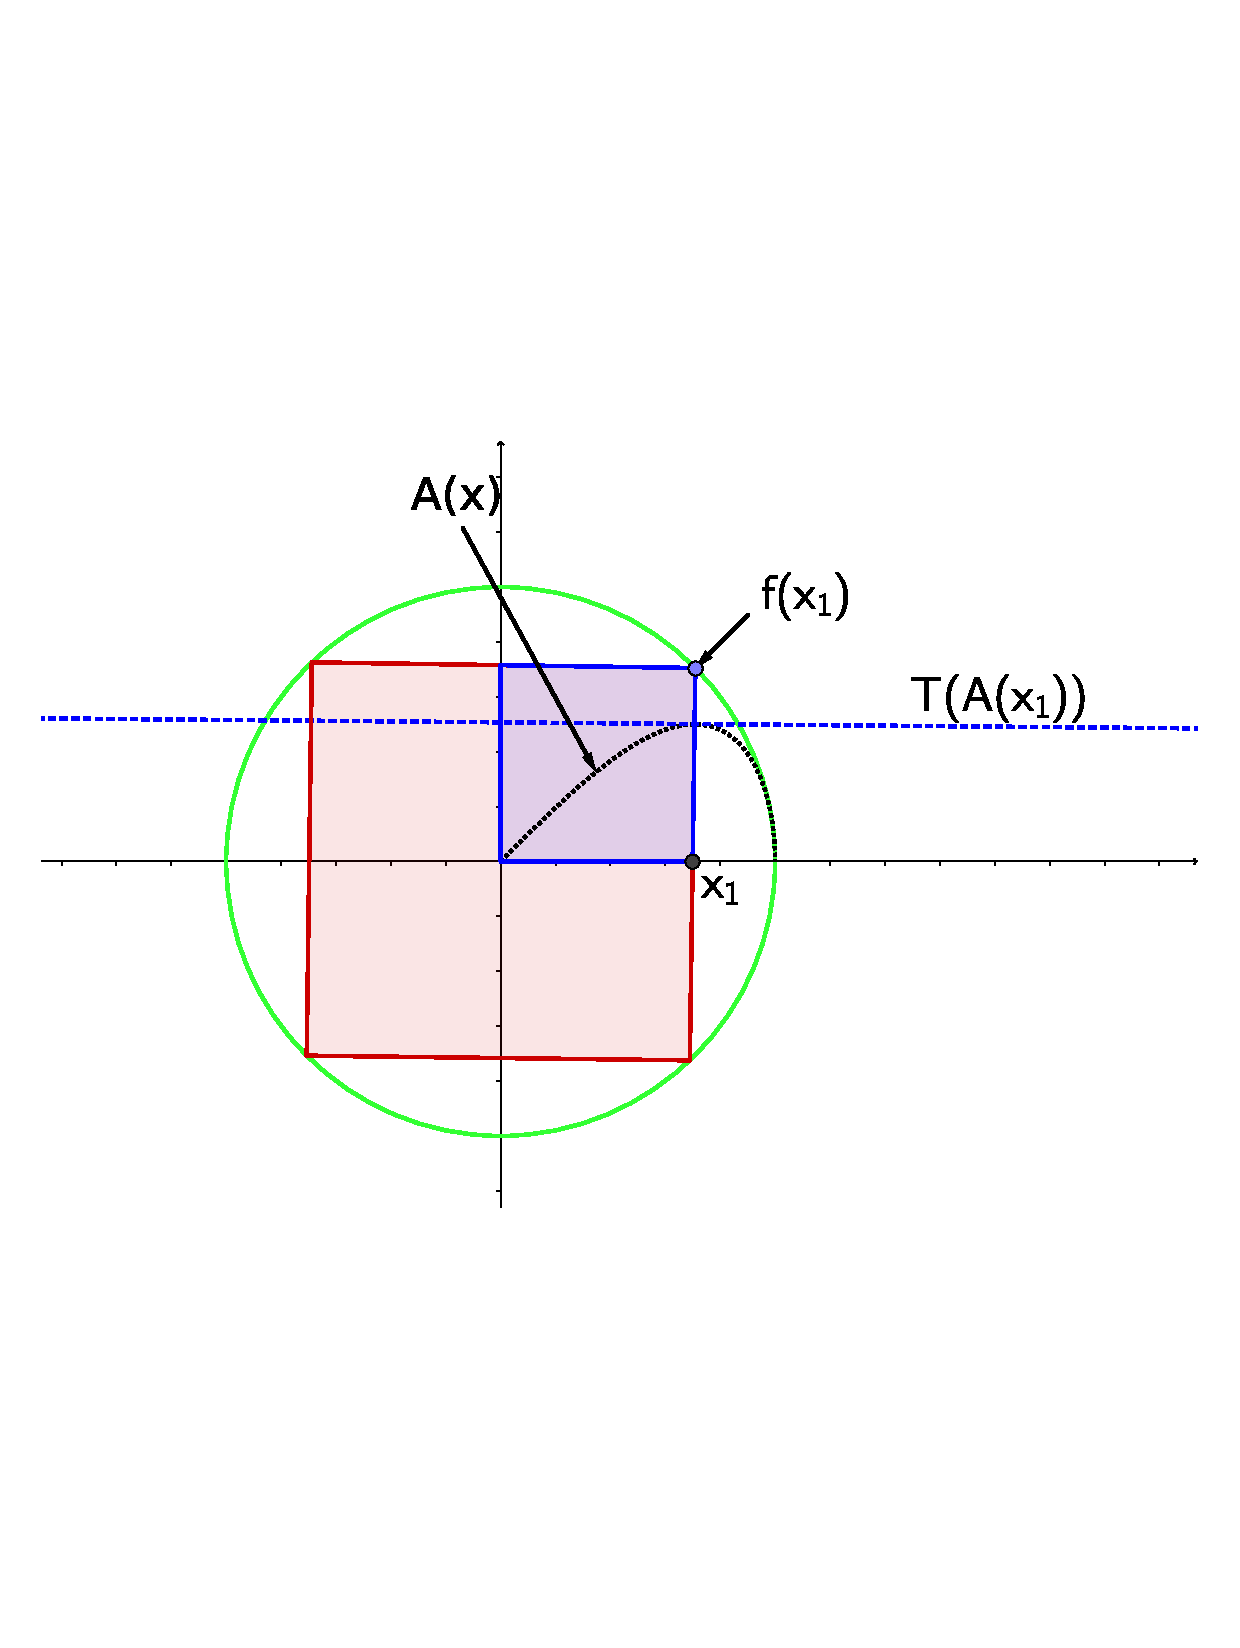
\includegraphics[width=0.8\textwidth]{bilder/maximale_flaeche.pdf}
\[a \cdot x^2 + b \cdot y^2 = c\]
Lösung:
\[A = 4 \cdot A_1\]
\[A_1 = x \cdot f(x)\]
\[\Rightarrow A = 4 \cdot x \cdot f(x)\]
% \[f(x) \stackrel{?}{=} \]
\[c = a \cdot x^2 + b \cdot y^2\]
\[\Rightarrow y = \left( \frac{c - a \cdot x^2}{b} \right)^{\frac{1}{2}}\]
\[A = 4 \cdot x \cdot \left( \frac{c - a \cdot x^2}{b} \right)^{\frac{1}{2}}\]
Wo ist $A_1$ maximal? \\
$\rightarrow$ Dort wo die Ableitung $0$ ergibt. 
\[A' \stackrel{!}{=} 0\]
\[A' = 4 \left(\frac{c - a \cdot x^2}{b}\right)^\frac{1}{2} + 4 \cdot x \left(\frac{1}{2} \cdot \left(\frac{c - a \cdot x^2}{b}\right)^{-\frac{1}{2}} \cdot \left(\frac{-2 \cdot a \cdot x}{b}\right)\right) = 0\]
\[A' = \left(\frac{c - a \cdot x^2}{b}\right)^{\frac{1}{2}} + x \cdot \left(\frac{1 \cdot \left(\frac{-2ax}{b}\right)}{2 \cdot \left(\frac{c - ax^2}{b}\right)^{\frac{1}{2}}}\right) = 0\quad \left|\text{mit }\left(\frac{c - ax^2}{b}\right)^{\frac{1}{2}} \right.\text{ erweitern}\]
\[A' = \frac{c - ax^2}{b} + x \cdot \frac{-ax}{b} = 0\]
\[A' = c - ax^2 - ax^2 = c - 2 \left(ax^2\right) = 0\]
\[c = 2 \left(ax^2\right)\]
\[\underline{x = \pm\sqrt{\frac{c}{2a}}}\]
$\rightarrow$ Weil die Fläche nur positiv sein kann, gilt nur $x \leq 0$
\[\Rightarrow A = 4 x \cdot f(x) = 4 x \left(\frac{c - ax^2}{b}\right)^{\frac{1}{2}}\]
\[A = 4 \sqrt{\frac{c}{2a}} \left(\frac{c - a \sqrt{\frac{c}{2a}}^2}{b}\right)^{\frac{1}{2}}\]
\[A = 4 \sqrt{\frac{c}{2a} \left(\frac{c - a \frac{c}{2a}}{b}\right)}\]
\[\underline{\underline{A = 2 \sqrt{\frac{c^2}{ab} } = \frac{2c}{\sqrt{ab}}}}\]
\section{Statue}
Aufgabenstellung: \\
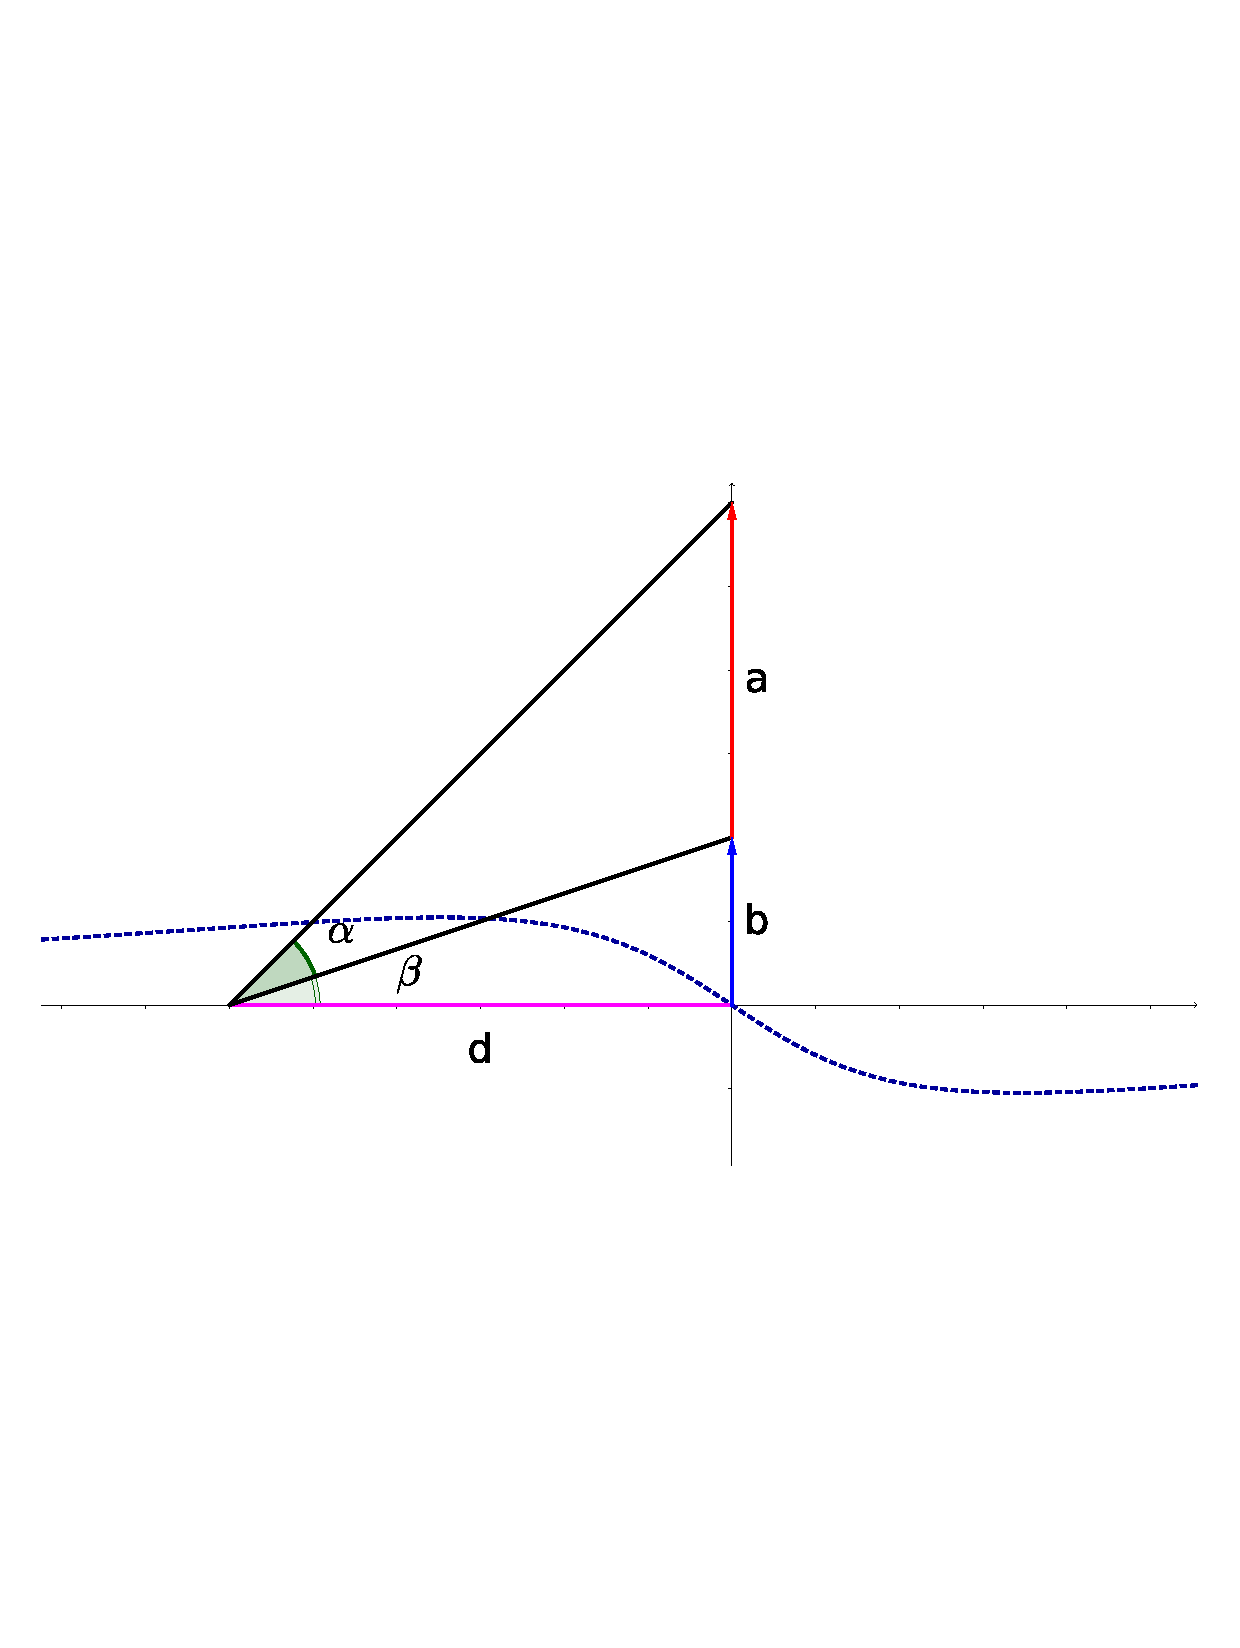
\includegraphics[width=0.8\textwidth]{bilder/statue.pdf}
\[ b = \text{Erde zu Statuenfuss} \]
\[ a = \text{Satuenfuss zu Statuenkopf} \]
\[ d = \text{Statue zu Betrachter} \]
\[ \alpha = \text{Winkel von Statuenkopf zu Statuenfuss} \]
Wo ist der Winkel $\alpha$ maximal? Dort wo die Ableitung der Funktion $\alpha(d)$ Null ergibt also $\alpha'(d)=0$ ist. 
Um dies zu bestimmen muss $\alpha$ definiert werden. 
Da dies auf Anhieb nicht möglich ist, kann man sich folgende Überlegung machen:
\[ \beta = \text{Winkel Betrachter zu Statuenboden} \]
\[ \gamma = \text{Winkel Betrachter zu Statuenkopf} \]
\[ \Rightarrow \gamma = \alpha + \beta \]
\[ tan(\gamma) = \tan(\alpha + \beta) = \left(\frac{a+b}{d}\right) \]
\[ \Rightarrow \alpha + \beta = arctan\left(\frac{a+b}{d}\right) \]
Nun haben wir eine neue Unbekannte $\beta$. Diese muss eliminiert bzw. substituiert werden durch etwas bekanntes oder gesuchtes.
\[ \tan(\beta) = \left(\frac{b}{d}\right) \rightarrow \beta = arctan\left(\frac{b}{d}\right) \]
\[ \Rightarrow \alpha = arctan\left(\frac{a+b}{d}\right) - \beta = arctan\left(\frac{a+b}{d}\right) - arctan\left(\frac{b}{d}\right) \]
\[ \alpha' \stackrel{!}{=} 0 \rightarrow \alpha' = \frac{-(a+b)}{d^2 + (a+b)^2} + \frac{b}{d^2 + b^2} = 0 \]
\[ \Rightarrow d = \sqrt{ab + b^2} \]
